\chapter{Tests}

\section{Funktionale Tests}\label{sec:tests-functional}

Für die Durchführung der funktionalen Tests wurde \textit{Postman} verwendet.\\

Während funktionale Tests darauf abzielen, die Korrektheit der Implementierung zu verifizieren, 
liegt der Fokus darauf, sicherzustellen, dass die \ac{API}-Endpunkte die spezifizierten Anforderungen 
in verschiedenen Anwendungsfällen korrekt erfüllen. Funktionale Tests umfassen unter anderem folgende Ziele:

\begin{itemize}
    \item Validierung der HTTP-Statuscodes
    \item Überprüfung der Struktur und Inhalte der Rückgaben
    \item Behandlung von Randfällen und fehlerhaften Anfragen
    \item Test von Autorisierungsmechanismen
\end{itemize}

\subsection{Postman}

\textit{Postman} ist ein \ac{API}-Client, der es ermöglicht, HTTP-Anfragen an eine \ac{API} zu senden und die Antworten zu überprüfen.
Es bietet eine grafische Benutzeroberfläche, um Anfragen zu erstellen und zu senden, sowie die Möglichkeit, Testfälle zu definieren und zu automatisieren.
Besonders nützlich ist die Möglichkeit, sogenannte \textit{Collections} zu erstellen, die mehrere Anfragen und Testfälle enthalten können, welche dann in 
einer Sequenz ausgeführt werden.
Diese \textit{Collections} können als \ac{JSON}-Dateien exportiert und geteilt werden, um Tests zu reproduzieren oder zu teilen.

\subsubsection*{Test Aufbau in Postman}

Jede Anfrage, Ordner, oder Collection in Postman kann mit sogennannten \textit{Pre-Request} und \textit{Post-Request} Skripten versehen werden, welche in JavaScript geschrieben sind.
Diese werden vor bzw. nach der eigentlichen Anfrage/Liste von Anfragen ausgeführt und können dazu verwendet werden, um Variablen zu setzen, oder die Antwort zu verarbeiten.
In den \textit{Post-Request} Skripten werden die Tests mit dem eingebauten Test-Runner von Postman geschrieben, welcher es ermöglicht, die Antwort auf verschiedene Kriterien zu prüfen.\\
Generel unterscheidet man zwischen zwei Arten von funktionalen Tests für \ac{API}s: \textit{Endpoint Monitoring} und \textit{Scenario Testing}.

\subsection{Endpoint Monitoring}

Beim \textit{Endpoint Monitoring} werden die Endpunkte der \ac{API} einzeln nach dem Schema der Spezifikation betrachtet. Es wird also für 
jeden Endpunkt ein Testfall erstellt, der die möglichen Statuscodes und Rückgabewerte überprüft. Zusätzlich wird auch die verwendete Authentifizierungsmethode überprüft.
Hierbei werden die \textit{Pre-Request} Skripte verwendet, um eventuelle Abhängigkeiten zwischen den Anfragen zu lösen, z.B. wird ein Post erstellt, 
damit für diesen ein Kommentar in der zu testenden Anfrage erstellt werden kann. \\
Als Beispiel wird der Endpoint \textit{PUT /posts/{{postId}}/comments/{{commentId}}} betrachtet, welcher einen Kommentar eines Posts bearbeitet.
Die möglichen Ergebnisse der Anfrage sind:
\begin{itemize}
    \item \textbf{200 OK} - Der Kommentar wurde erfolgreich bearbeitet
    \item \textbf{401 Unauthorized} - Der Benutzer ist nicht autorisiert
    \item \textbf{404 Not Found} - Der Kommentar oder der Post existiert nicht
\end{itemize}

\subsubsection*{200 OK}

Damit die Anfrage ausgeführt werden kann, muss jeweils ein Nutzer, ein Post und ein Kommentar erstellt werden. Dies wird in den \textit{Pre-Request} Skripten erledigt.
Wie in Listing~\ref{lst:pre-request-script-200} zu sehen, wird zuerst ein Nutzer erstellt, dann ein Post und schließlich ein Kommentar. Dazu werden die
benötigten Strings, wie Nutzername, Email, Titel und Inhalt des Posts, sowie der Inhalt des Kommentars, generiert. Diese werden dann in den Anfragen verwendet, welche 
den entsprechenden Nutzer, Post und Kommentar erstellen. Die IDs der erstellten Objekte werden in Variablen gespeichert, um sie in der eigentlichen Anfrage zu verwenden. 
Der Body der Anfrage enthält den neuen Inhalt des Kommentars, welcher im \textit{Pre-Request} Skript als Variable erstellt wurde (Listing~\ref{lst:request-body-200}). Die Authorisierung erfolgt über einen \textit{\ac{API}-Key}, welcher in einer Variable
gespeichert ist (Abbildung~\ref{fig:authorization-postman}).

\begin{lstlisting}[caption=Request Body für die Bearbeitung eines Kommentars,label=lst:request-body-200]
{
    "content": "{{updatedCommentContent}}",
    "authorId": {{userId}}
}
\end{lstlisting}

\begin{figure}[htpb]
    \centering
    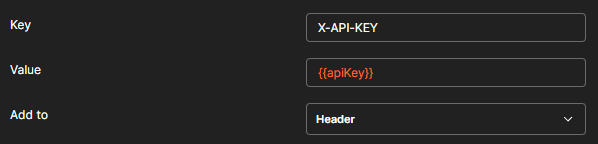
\includegraphics[width=0.7\textwidth]{Graphics/postmanauthscreen.png}
    \caption{Authentifizierung in Postman}
    \label{fig:authorization-postman}
\end{figure}

Zum Testen der Anfrage wird im \textit{Post-Request} Skript ein Testfall erstellt, welcher die Antwort auf den Statuscode 200 OK überprüft. Außerdem wird bestätigt, 
dass der Inhalt des Kommentars aktualisiert wurde (Listing~\ref{lst:post-request-script-200}). 

\begin{lstlisting}[language=JavaScript, caption=\textit{Post-Request} Skript für die Bearbeitung eines Kommentars,label=lst:post-request-script-200]
pm.test("Status code is 200", function () {
    pm.response.to.have.status(200);
});

// Test to check if the response contains updated comment data
pm.test("Response contains updated comment data", function () {
    var jsonData = pm.response.json();
    pm.expect(jsonData).to.have.property("id", parseInt(pm.collectionVariables.get("commentId")));
    pm.expect(jsonData).to.have.property("content", pm.collectionVariables.get("updatedCommentContent"));
    pm.expect(jsonData).to.have.property("authorId", parseInt(pm.collectionVariables.get("userId")));
    pm.expect(jsonData).to.have.property("postId", parseInt(pm.collectionVariables.get("postId")));
});
\end{lstlisting}

\subsubsection*{401 Unauthorized}

Um den Statuscode 401 Unauthorized zu testen, wird die Anfrage mit dem falschen \textit{\ac{API}-Key} gesendet. Zum Schluss muss dann nur der Statuscode getestet werden (Listing~\ref{lst:post-request-script-401}).

\begin{lstlisting}[language=JavaScript, caption=\textit{Post-Request} Skript für 401 Unauthorized,label=lst:post-request-script-401]
pm.test("Status code is 401", function () {
    pm.response.to.have.status(401);
});
\end{lstlisting}

\subsubsection*{404 Not Found}

Um den Statuscode 404 Not Found zu testen, wird die Anfrage einmal mit ungültiger Post-ID und einmal mit ungültiger Kommentar-ID gesendet. 
Die Tests sind identisch zu denen für 401 Unauthorized, nur dass der Statuscode 404 getestet wird (Listing~\ref{lst:post-request-script-404}).

\begin{lstlisting}[language=JavaScript, caption=\textit{Post-Request} Skript für 404 Not Found,label=lst:post-request-script-404]
pm.test("Status code is 404", function () {
    pm.response.to.have.status(404);
});
\end{lstlisting}

\subsection{Scenario Testing}

Beim \textit{Scenario Testing} werden mehrere Endpunkte in einer Sequenz getestet, um die Funktionalität der \ac{API} in verschiedenen Anwendungsfällen zu überprüfen. 
Dies ist oft bei komplexeren Anwendungsfällen nützlich, bei denen mehrere Endpunkte zusammenarbeiten müssen, um das gewünschte Ergebnis zu erzielen. 
So können besonders kritische Pfade in der \ac{API} getestet werden, um sicherzustellen, dass sie korrekt funktionieren. 
Dies ist vor allem notwendig bei Anwendungen, die auf einer umfangricheren \ac{API} basieren, wie z.B. Webanwendungen oder mobile Apps.
Ein Beispiel für ein simples Szenario wäre das ``Erstellen und Abrufen eines Posts'':

\begin{enumerate}
    \item \textbf{Ein Nutzer erstellt einen Post} - \textbf{POST /posts}
        \begin{itemize}
            \item existiert der Nutzer?
            \item sind alle Parameter vorhanden?
            \item ist der Inhalt des Posts valide?
            \item wird der Post erstellt?
        \end{itemize}
    \item \textbf{Der erstellte Post wird abgerufen} - \textbf{GET /posts/{{postId}}}
        \begin{itemize}
            \item existiert der Post?
            \item ist der Inhalt des Posts korrekt?
        \end{itemize}
    \item \textbf{Der erstellte Post wird gelöscht} - \textbf{DELETE /posts/{{postId}}}
        \begin{itemize}
            \item wird der Post gelöscht?
        \end{itemize}
\end{enumerate}

Da die \ac{API} in diesem Projekt relativ einfach ist, wurden keine komplexen Szenarien getestet, sondern nur die einzelnen Endpunkte.

\subsection{Automatisierung und Variablen}

Um eine effiziente Testausführung zu gewährleisten, wurden in Postman Variablen verwendet, 
um Werte wie \textit{postId} und \textit{authorId} zwischen den Testläufen dynamisch zu speichern. 
Dies ermöglichte eine Automatisierung der Testsequenzen, bei denen Ergebnisse aus einem Testlauf in den nächsten übernommen wurden. 
Zudem konnten Fehler bei ungültigen Eingaben erkannt werden, z.B. bei fehlenden Parametern oder unzulässigen Datentypen.
Die Verwendung von Postman ermöglichte die Durchführung dieser Tests sowohl manuell als auch automatisiert,
wobei alle Testfälle erfolgreich durchlaufen wurden und die Funktionalität der \ac{API} bestätigten.
Für die automatisierte Ausführung der Tests wurde eine \textit{\ac{CI}} Pipeline in Github Actions erstellt, welche bei jedem Push ausgeführt wird (siehe Continous Integration~\ref{sec:CI})./

\subsection{Bewertung}

Postman erweist sich als ein benutzerfreundliches und leistungsstarkes Werkzeug für API-Tests. 
Es bietet eine Vielzahl von Funktionen, die die Erstellung, Ausführung und Automatisierung von Tests erleichtern. 
Besonders hervorzuheben ist die Möglichkeit, Variablen zu verwenden, 
um Werte wie \textit{postId} und \textit{authorId} zwischen den Testläufen dynamisch zu speichern.
Außerdem ist die Vielseitigkeit von \textit{Collections} zur Strukturierung und Organisation von Testfällen sehr nützlich.
Dies ermöglicht eine effiziente und automatisierte Testausführung. 
Zudem können Fehler bei ungültigen Eingaben, wie fehlenden Parametern oder unzulässigen Datentypen, leicht erkannt werden.

Allerdings bringt das Always-Online-Modell von Postman auch einige Nachteile mit sich. 
Die ständige Abhängigkeit von der Postman API kann störend sein, insbesondere bei der Integrierung in \ac{CI}/\ac{CD}-Pipelines.
Zudem schränkt das Bezahlmodell die Anzahl der täglichen Testausführungen in der kostenlosen Version ein, 
was bei umfangreicheren Projekten zu erheblichen Einschränkungen führen kann.

Angesichts dieser Einschränkungen wäre es sinnvoll, für zukünftige Entwicklungen auch alternative Tools in Betracht zu ziehen. 
Tools wie \textit{Newman}, die CLI-Version von Postman, welche in der \ac{CI} Pipeline des Projekts verwendet wurde,
war hier eine nötige Ergänzung.

Anndere API-Testwerkzeuge wie \textit{Hoppscotch} könnten eine gute Alternative darstellen, 
um die Abhängigkeit von der Postman Struktur zu reduzieren und die Flexibilität bei der Testausführung zu erhöhen.

Insgesamt bietet Postman eine solide Grundlage für API-Tests, 
jedoch sollten die genannten Einschränkungen bei der Planung und Durchführung von Tests berücksichtigt werden.


\clearpage
\section{Load Tests}\label{sec:tests-load}
Zur Umsetzung des Load Testings wurde Apache JMeter eingesetzt.\\

Während funktionale Tests die Korrektheit der Implementierung prüfen,
evaluieren Load Tests die Performance des Systems unter hoher Last,
beispielsweise bei vielen nebenläufigen Zugriffen.
Es gibt zahlreiche Gründe eine Anwendung Load Tests zu unterziehen.
Diese sind unter anderem:

\begin{itemize}
    \item Messung der Systemperformance
    \item Identifikation von Bottlenecks
    \item Untersuchung der Skalierbarkeit des Systems
    \item Entdeckung von Race Conditions
\end{itemize}

\subsection{Starten von JMeter}

JMeter kann im GUI- oder CLI-Modus gestartet werden.
Der GUI-Modus wird zum Erstellen und Debuggen von Tests eingesetzt,
welche anschließend im CLI-Modus ausgeführt werden können.

JMeter startet standardmäßig im GUI-Modus.
Um Tests im CLI-Modus auszuführen, kann folgender Befehl eingesetzt werden.

\begin{lstlisting}[caption=Beispielkonfiguration des CLI-Modus]
    jmeter -n -t testplan/TestPlan.jmx -l "results/result.jtl" -j "logs/logs.log" -eof reports/
\end{lstlisting}

Die eingesetzten Optionen haben folgende Bedeutung:

\begin{itemize}
    \item \texttt{-n} - CLI-Modus
    \item \texttt{-t} - Pfad zum Testplan
    \item \texttt{-l} - Pfad zur Testlogdatei (Testergebnisse)
    \item \texttt{-j} - Pfad zur Jmeterlogdatei (Informationen über Testausführung und aufgetretene Fehler)
    \item \texttt{-e} - Report generieren
    \item \texttt{-o} - Pfad für Reportdateien
    \item \texttt{-f} - Alte Ergebnisse und Reports löschen
\end{itemize}

\subsection{Erstellung von Testplänen}

Tests werden in Form eines Testplans geschrieben.
Ein Testplan ist ein Baum, der Elemente aus verschiedenen Kategorien enthalten kann (siehe \url{https://jmeter.apache.org/usermanual/test_plan.html}).

\begin{itemize}
    \item Thread Groups kontrollieren wie oft Sampler ausgeführt werden, insbesondere wie viele Anfragen nebenläufig stattfinden.
    \item Logic Controller beeinflussen die Ausführungsreihenfolge der Sampler.
    \item Sampler enthalten die auszuführenden Tests, z.B. HTTP-Anfragen.
    \item Listener speichern die Ergebnisse eines Samplers und können diese im GUI-Modus grafisch aufbereiten.
    \item Configuration Elements stellen Daten für Tests zur Verfügung, unter anderem durch Definition von Konstanten,
          Erzeugung zufälliger Werte oder Einlesen externen Dateien.
\end{itemize}

%\vspace{2em}

Die Elemente können auf unterschiedliche Weise verschachtelt werden, gängig ist dabei folgende Reihenfolge:

\begin{itemize}
    \item Der Testplan enthält \texttt{Thread Groups}, wobei jeder Thread einer Gruppe einen User darstellt.
    \item \texttt{Thread Groups} enthalten \texttt{Sampler}, welche von jedem Thread der Gruppe von oben nach unten ausgeführt werden.
    \item \texttt{Samplers} enthalten (einen) Listener, welcher die Ergebnisse aufzeichnet und im GUI-Modus visualisieren kann.
    \item \texttt{Configuration Elements} werden nach Bedarf als Kinder von \texttt{Thread Groups}, 
    \texttt{Samplers} oder dem Wurzelelement des Testplans definiert.   
\end{itemize}

\begin{figure}[h]
    \centering
    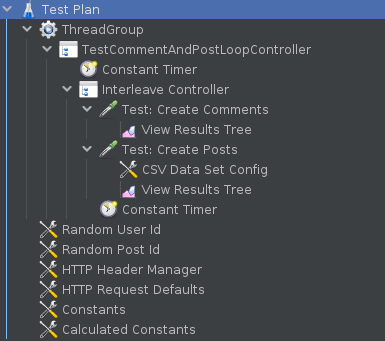
\includegraphics[width=0.65\linewidth]{Graphics/Testplan.png}
    \caption{Beispiel eines Testplans}
\end{figure}

\subsection{Report Dashboard}\label{sec:Dashboard}

JMeter kann die erfassten Leistungsparameter in einem HTML-Dashboard zusammenfassen. 
Dieses besteht aus verschiedenen Graphen, welche etwa Antwortzeiten und Datendurchsatz über den Verlauf des Tests darstellen.
Um einen Report zu generieren, muss die Option \texttt{-e} benutzt werden.
Das Dashboard ist direkt ohne weitere Konfiguration benutzbar und sollte für die meisten Projekte ausreichend sein.
Nur in fortgeschritteneren Anwendungsfällen, etwa zur automatischen Auswertung, 
ist die Verwendung von Listenern mit eigenen Result-Dateien notwendig.

JMeter unterstützt Anpassungen an der Graphgenerierung, etwa die Anpassung der zeitlichen Auflösung.
Weiterhin können eigene Graphen hinzugefügt werden. 
Siehe hierzu \url{https://jmeter.apache.org/usermanual/generating-dashboard.html}.

Ein Beispielreport befindet sich im Ordner \texttt{jmeter/ReportBeispiel}.



\subsection{Verwendung von Variablen und Scripting}

JMeter ermöglicht die Definition von Variablen und Skripten, um Tests besser wart- und anpassbar zu machen.

Zur Definition von Variablen kann etwa das Configuration Element \texttt{User Defined Variables} eingesetzt werden.
In diesem Element definierte Konstanten können grundsätzlich mit der Syntax \lstinline|${Variablenname}| referenziert werden,
was allerdings nicht von allen Eingabefeldern unterstützt wird.
So funktioniert dies etwa im Körper einer HTTP Request oder zur Angabe der Wiederholungen einer Threadgroup,
nicht aber zur Angabe von Dateipfaden für Sampler.

JMeter unterstützt mehrere Skriptinterpreter (Beanshell, Groovy, Javascript, Jexl). 
Die Dokumentation empfiehlt die Verwendung von Groovy oder Jexl3.
Skripte können statt Literalen zur Definition verschiedener Parameter des Testplans eingesetzt werden.
Die Syntax zur Ausführung von Skripten folgt diesem Schema: \lstinline|${__interpreter(script)}|.

Wird die Verwendung einer Variable mittels \lstinline|${Variablenname}| nicht direkt unterstützt,
kann der Wert der Variable oftmals durch ein Skript ausgelesen werden.
Hierzu kann darin die Funktion \lstinline{vars.get("Variablenname")} benutzt werden.
Leider funktioniert auch dieser Ansatz nicht in allen Fällen.

Scripting ermöglicht die Berechnung von Konstanten in Abhängigkeit von anderen Konstanten.
Die abhängige Konstante muss in einem eigenen \texttt{User Defined Variables}-Element definiert werden.
Dieses muss sich im Baum unter dem ursprünglichen Konfigurationselement befinden.
Wird die Konstante im gleichen Element oder einem im Baum höherstehenden Element definiert,
scheitert die Auflösung der abhängigen Variable und sie wird als leerer String behandelt.

\begin{lstlisting}[caption=Beispiel eines Groovy-Skripts]
    ${__groovy(
        vars.get("UserCount").toInteger() 
        * vars.get("PostsPerUserCount").toInteger()
    )}
    \end{lstlisting}

Um Fehler beim Einsatz von Variablen zu untersuchen,
kann der Sampler \texttt{Debug Sampler} eingesetzt werden.
Dieser wertet bei Ausführung alle verfügbaren Variablen aus, sodass deren Werte überprüft werden können.
Die Werte sind im GUI-Modus unter \texttt{Response Data} des zum Sampler hinzugefügten Listener einsehbar.

\subsection{Relative Pfade}

JMeter bietet keine vollständige Unterstützung für relative Pfade.

Die Angabe relativer Pfade ist im GUI-Modus nicht möglich.
Ersetzt man im durch den GUI-Modus erzeugten Testplan, einer XML-Datei, absolute durch relative Pfade,
so werden diese im CLI-Modus korrekt aufgelöst.
Öffnet man den manipulierten Testplan erneut im GUI-Modus,
kann JMeter die relative Pfade jedoch nicht auflösen.

Um trotzdem absolute Pfade zu vermeiden, 
kann ein Basispfad als Variable definiert werden.
Pfade werden dann als Konkatenation dieser Variable und des gewünschten relativen Pfades definiert.
Der Basispfad kann als Literal oder durch ein Skript definiert werden.

\begin{lstlisting}[caption=Ermitteln des Working Directory\protect\footnotemark]
    ${__BeanShell(
        import org.apache.jmeter.services.FileServer; 
        FileServer.getFileServer().getBaseDir();
    )}
    ${__BeanShell(File.separator,)}
\end{lstlisting}
\footnotetext{Quelle:\url{https://stackoverflow.com/questions/11268015}}

\section{Continuous Integration}\label{sec:CI}

\textit{Die \ac{CI}-Definitionen liegen im Verzeichnis} \texttt{.github/workflows}.\\

Da wir nun alle Tests geschrieben haben, wollen wir dass diese automatisiert ausgeführt werden und Reports geben zum aktuellen Stand der Implementierung im Repository. Dazu benutzen wir \textbf{Github Actions}. Diese konfigurieren wir so, dass alle Tests (siehe \ref{sec:tests-functional} und \ref{sec:tests-load}) automatisch bei einem Git-Push auf das Repository ausgeführt werden.

Sollten Tests fehlschlagen wird dies automatisch durch diese Pipeline festgestellt und benachrichtigt den Autor des Commits.
Des Weiteren generiert der Workflow für die Load-Tests einen HTML-Report mit Performance-Indikatoren und Graphen (siehe \ref{sec:Dashboard}).
